\documentclass[a4paper, 12pt]{article}
\usepackage{amsmath, amsfonts, amsthm, amssymb}
\usepackage{color, fullpage, hyperref}
\usepackage{graphicx}
\graphicspath{{./img/}}

\setlength{\parindent}{0pt}
\begin{document}
\textbf{Name: Jiaming Lu $~~~~~~~~~~~~~~~~~~~~~~~~~
~~~~~~~~~~~$ Student number: 1008494620}

Solutions:
\begin{enumerate}
	\item WLOG:

		Fix a point $p$ to an arbitrary position on the perimeter, 
		denotes the spherical distance between the other point, $q$, 
		by $d(p,q)$.
		To pick the location of $q$, we can either pick is from the left side 
		of $p$, in which within the interval $(p-\frac{\pi}{3},p]$, or from the 
		right side of $p$, in which within the $[p,p+\frac{\pi}{3})$.

		It is clear that the length of the intervals mentioned above is 
		$\frac{\pi}{3}$, so we have
		$$\begin{aligned}
			P(d(p,q) < \frac{\pi}{3}) 
			&= \frac{\pi/3+\pi/3}{2\pi \cdot 1}\\
			&= \frac{1}{3}
		\end{aligned}$$
	\item 
	\begin{enumerate}
		\item 
		By the definition of exponential distribution
		$$\begin{aligned}
			P(X<5000) 
			&= \int^{5000}_{-\infty} \lambda e^{-\lambda x} dx\\
			&= \int ^{5000}_{0}\frac{1}{8267} e^{-x/8267} dx\\
			&= 0.45382
		\end{aligned}$$
		\item 
			Still, by definition,
		$$\begin{aligned}
			P(X\leq m) &= \frac{1}{2}\\
			\int^{m}_{-\infty} \lambda e^{-\lambda x}dx &= \frac{1}{2}\\
			\int^{m}_{0} \frac{1}{8267} e^{-\frac{x}{8267}} dx &= \frac{1}{2}\\
			1-e^{-\frac{n}{8267}} &= \frac{1}{2}\\
			m &= 5730.2
		\end{aligned}$$
	\end{enumerate}

	\newpage
	\item 
		\begin{enumerate}
			\item 
	Verifying if the CDF is valid:
	\begin{itemize}
		\item $
				\lim _{x\to\infty}F(x)
				=\lim _{x\to\infty} 1-\frac{1}{x}
				= 1-0
				= 1$
		\item
			$\lim_{x\to -\infty}F(x) = \lim_{x\to-\infty}0 = 0$
		\item 
			Pick two arbitrary $x_1,x_2\in\mathbb{R},~ s.t.~ x_1<x_2$, we have 
			three cases.

			\textbf{Case 1:} $x_1,x_2 \leq 1$

			$f(x_1) = f(x_2) = 0$, so we have $f(x_1)\leq f(x_2)$ as wanted.

			\textbf{Case 2:} $x_1\leq 1, x_2>1$

			By definition, we have $f(x_1) = 0$. And also,
			$$\begin{aligned}
				x_2 &> 1\\
				\frac{1}{x_2}&<1\\
				1-\frac{1}{x_2}&>0\\
				f(x_2)&>0 = f(x_1)
			\end{aligned}$$
			As wanted.

			\textbf{Case 3:} $x_1, x_2 > 1$
			$$\begin{aligned}
				x_1 &< x_2\\
				\frac{1}{x_1}&> \frac{1}{x_2}\\
				1-\frac{1}{x_1} &< 1-\frac{1}{x_2}\\
				f(x_1) &< f(x_2)
			\end{aligned}$$
			As wanted.


	\end{itemize}
		Plot of CDF:
		\begin{wrapfigure}
		\begin{center}
		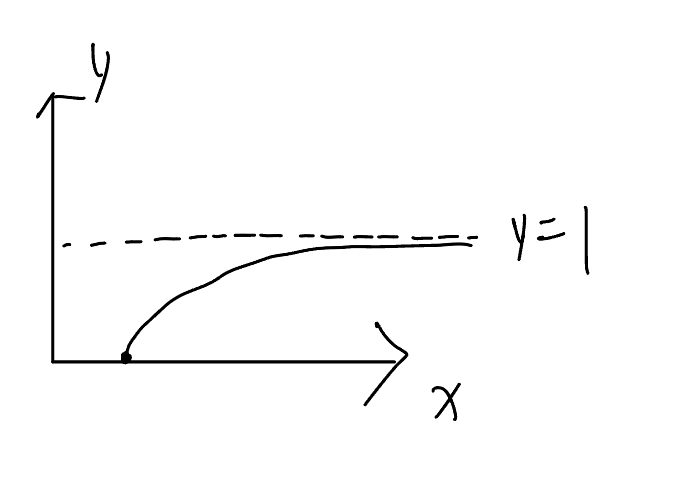
\includegraphics[width = 8cm]{img/q5_3_a.jpeg}
		\end{center}
		\end{wrapfigure}
	
	\item 
		By the definition of PDF,
		$$
		\begin{aligned}
			f(x) &= \frac{d}{dx}F(x) \\
				 &= 
		\begin{cases}
			\frac{d}{dx}0, 			&x\leq 1\\
			\frac{d}{dx}(1-1/x), 	&x>1
		\end{cases}\\
		&=
		\begin{cases}
			0, 		&x\leq 1\\
			1/x^2, 	&x>1
		\end{cases}
		\end{aligned}$$

		Plot of PDF:

		\begin{wrapfigure}
		\begin{center}
		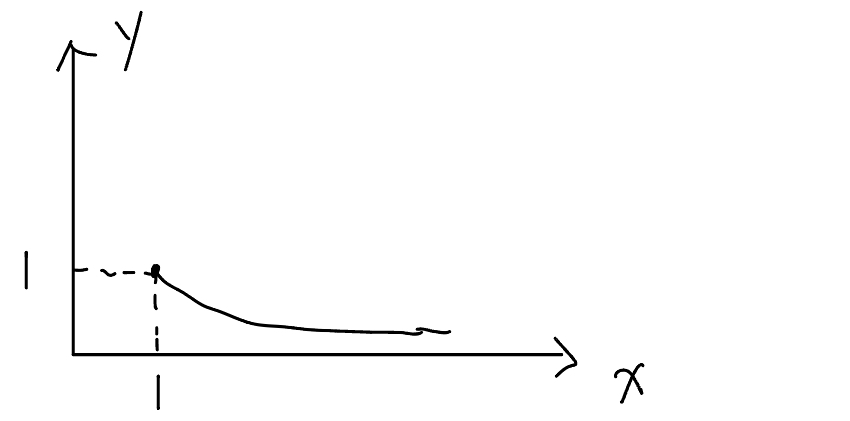
\includegraphics[width = 8cm]{img/q5_3_b.jpeg}
		\end{center}
		\end{wrapfigure}
	\end{enumerate}
\end{enumerate}
\end{document}
